\documentclass[runningheads]{llncs}
\bibliographystyle{splncs04}

\usepackage{glossaries}

% DEFINE ACRONYMS HERE. Params: label, short version, long version
\newacronym{CNN}{CNN}{Convolutional Neural Network}
\newacronym{CC}{CC}{Color Constancy}


\usepackage{Paper}


\graphicspath{ {./images/} }

\begin{document}

\title{An Investigation of Color Constancy for Image Classification}
\titlerunning{Color Constancy Classification}

\author{
    Uzairu Abubakar\inst{1} \and
    Niklas Bieck\inst{1} \and
    Fabiano Junior Maia Manschein\inst{1} \and
    Yuya Takagi\inst{1} \and
    Damien Muselet\inst{1}\orcidID{0000-0001-7803-1171}
}
\authorrunning{U. Abubakar et al.}

\institute{
    Université Jean Monnet Saint-Étienne, 10, rue Tréfilerie – CS 82301, 42023 Saint-Etienne Cedex 2, France
    \email{https://www.univ-st-etienne.fr/fr/index.html}
}



\maketitle

\begin{abstract}
    Color constancy, the process of determining the true color of light in an image
    and adjusting it to match a reference illuminant, is a widely researched area.
    A key argument in favor of this technique is its potential to enhance the training
    of other image processing techniques by eliminating the need to learn variations
    caused by different lighting conditions. To validate this claim, we conduct a
    comprehensive analysis by comparing the performance and training times of image
    classification models using a dataset of flower images. They are particularly
    suitable for this study due to the crucial role of color in their identification.
    The comparison is conducted with and without the application of color constancy
    methods as a preprocessing step. We also compare the results with the use of batch
    normalization as an alternative to color constancy.
    Our results show no particular gain made by our methods, but we believe further research
    is warranted.
\end{abstract}

% Here's my suggested structure for the paper. Subject to change, specially titles.
\section{Introduction}

\gls{CC} is a natural part of the human visual system that lets us recognize that a color
stays the same even under changing illumination. Letting computers do this same thing and then
modify the image color to represent their appearance under a neutral light source is a well-established
and on-going area of research. One of the presumed benefits of doing this is improved performance
of recognition tasks that rely to a large part on color, as it removes the need for the classification
model to learn to recognize objects under changing lighting conditions.

While some effort has been made to investigate how \gls{CC} correction can aid in video tracking
\cite{Agarwal2006}, as far as we can tell, no investigation specific to the field of object
classification has, as of yet, been performed. In this paper, we will do just that, using the
classification of flowers as a sample task, since this is clearly an area where color is of large
importance to a successful classification.

% Todo:
%! 1- lots of use of 'this'. Can the sentence be rewritten to be clearer?
%! 2- the use of terms such as 'as far as we know' and 'clearly' is dangerous. Alternatives?
%! 3- 'While some effort has been made...' -> 'While efforts to investigate... have been made, as far as...'  % Introduction
\section{Related studies}  % Previous related studies on applying CC as preprocessing
% This section is for the experiment part of the paper, where we talk about the
% pipeline, datasets, and the models we used.

% Suggested structure:
% 1- Experiment setup/structure (pipeline)
% 2- Datasets
% 3- CC models
% 4- CLF models

\section{Experiment}

\subsection{Datasets}

We used the publicly available Oxford 17 \cite{Nilsback06} and Oxford 104 \cite{Nilsback08} datasets. By using only existing datasets, we ensure that our results can more 
easily be contrasted with other research in this area.
 
\subsection{Color Constancy}

\begin{figure}
    \centering
    \begin{tabular}{c|cccc}
    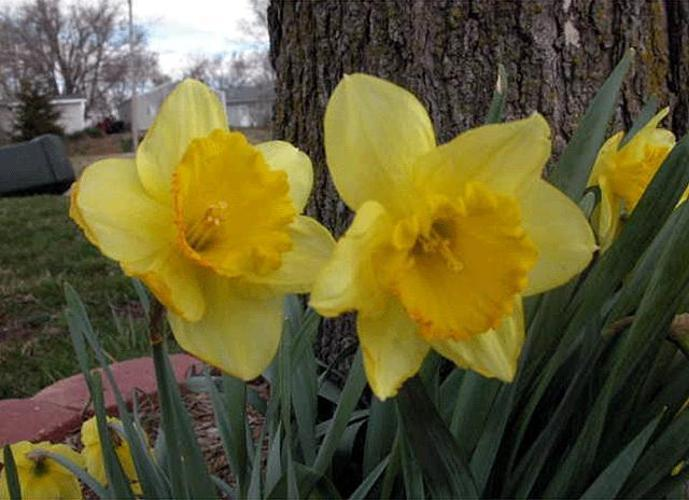
\includegraphics[width=0.165\textwidth]{cc_demo/flower001_base.png}&
    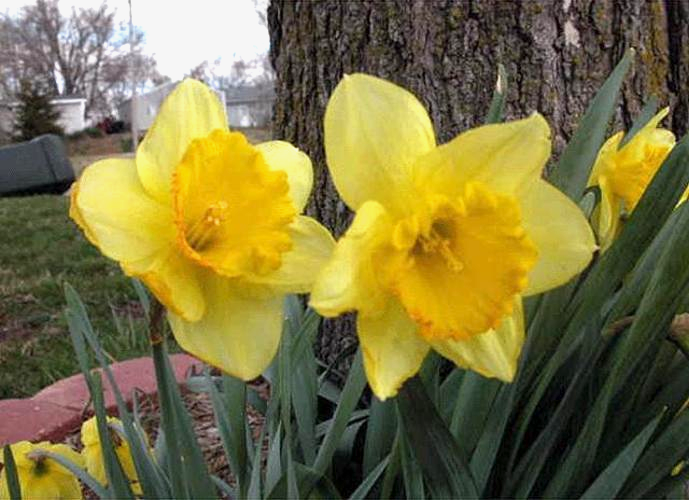
\includegraphics[width=0.165\textwidth]{cc_demo/flower001_whitePatch.png}&
    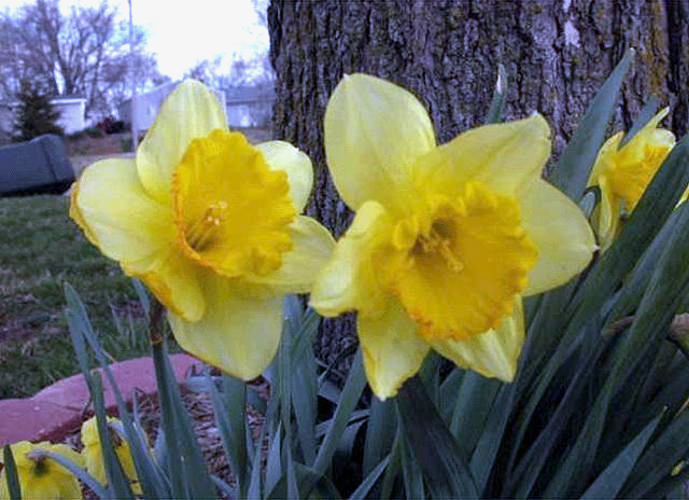
\includegraphics[width=0.165\textwidth]{cc_demo/flower001_greyWorld.png}&
    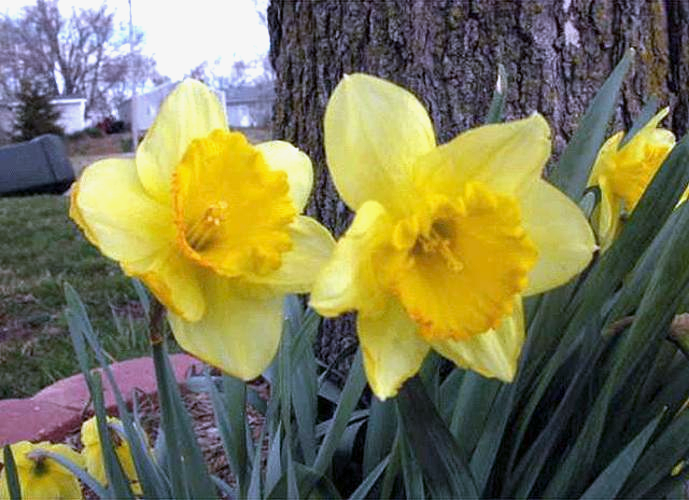
\includegraphics[width=0.165\textwidth]{cc_demo/flower001_grayEdge.png}&
    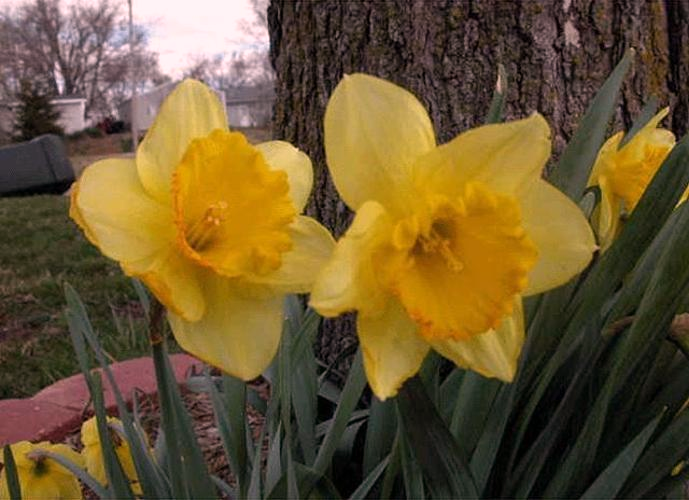
\includegraphics[width=0.165\textwidth]{cc_demo/flower001_fc4.png}\\
    (a)&(b)&(c)&(d)&(e)\\
    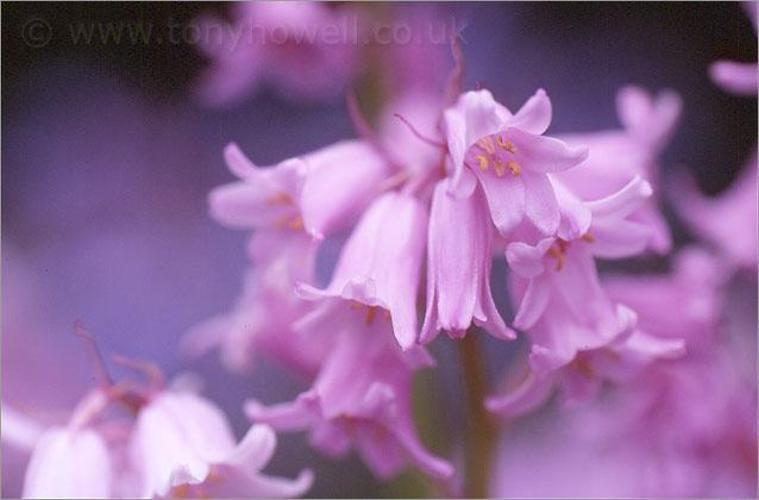
\includegraphics[width=0.165\textwidth]{cc_demo/flower268_base.png}&
    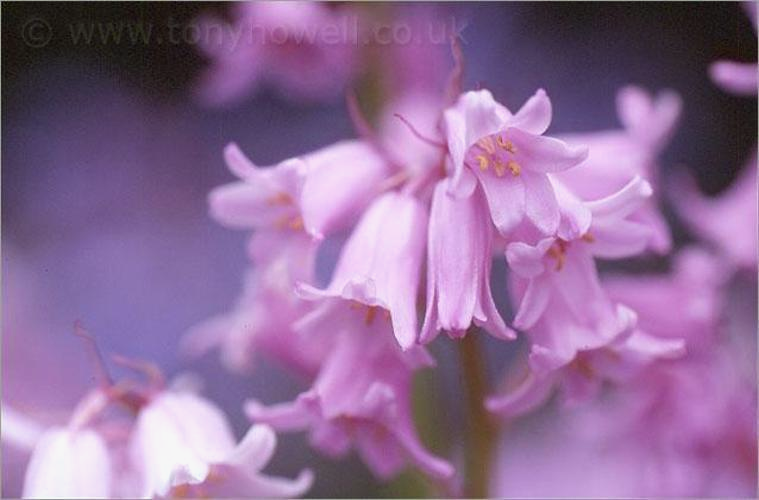
\includegraphics[width=0.165\textwidth]{cc_demo/flower268_whitePatch.png}&
    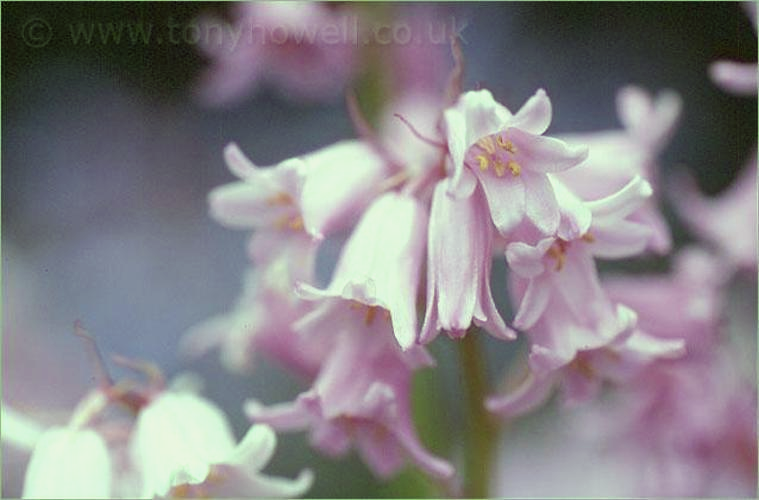
\includegraphics[width=0.165\textwidth]{cc_demo/flower268_greyWorld.png}&
    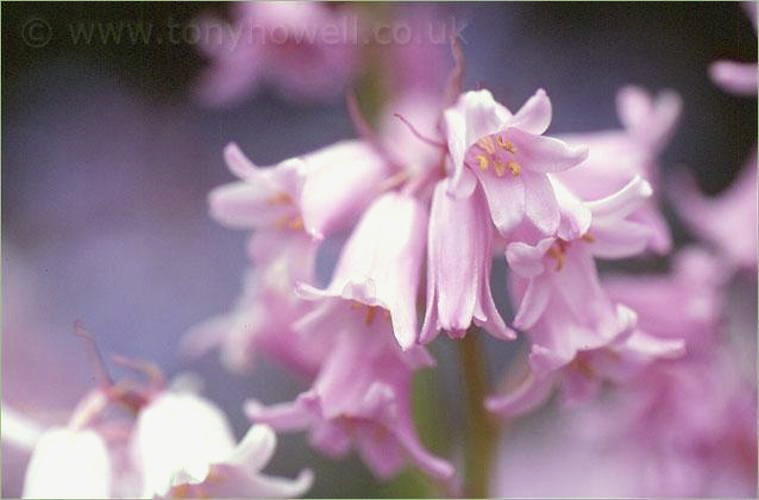
\includegraphics[width=0.165\textwidth]{cc_demo/flower268_grayEdge.png}&
    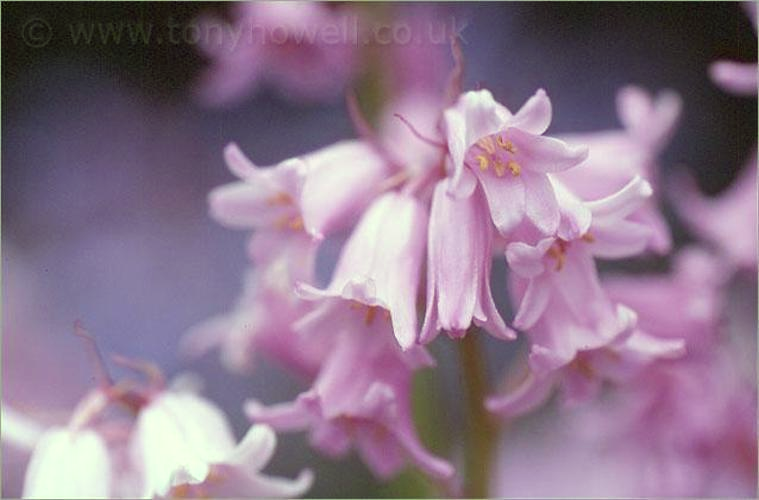
\includegraphics[width=0.165\textwidth]{cc_demo/flower268_fc4.png}\\
    (f)&(g)&(h)&(i)&(j)
    \end{tabular}
    \caption{A comparison of color constancy algorithms: (a) and (f): Original image.
        (b) and (g): White Patch. (c) and (h): Grey-World. 
        (d) and (i): Grey-Edge. (e) and (j): FC\textsuperscript{4}}
    \label{fig:cc_comparison}
\end{figure}

In order to have a wider spread of examined methods, we both make use of state-of-the art 
learning based methods (in this case represented by FC\textsuperscript{4}\cite{hu2017fc}), as well as classical simpler methods 
like White-Patch, Grey-World \cite{EbnerConstancy} and Grey-Edge \cite{van2005color}.
A comparison of these can be found in \ref{fig:cc_comparison}.

\subsubsection{Statistical Methods}

In the grey world algorithm, the assumption is made that the average reflectance of the scene should
be a shade of grey. We can therefore infer that any deviation of the average color from this grey tone stems from
the illumination in the scene. By simply dividing this out, we receive a color-corrected image.

White-Patch is a close relative of this method, where instead we assume that the brightest spot in the image (for each channel)
is representative of the overall light color.

In the grey-edge hypothesis we instead assume that the average image gradient can be used as an indication of the light color.

All of these algorithms were reimplemented by us. Notably, based on the recommendation made by Ebner \cite{EbnerConstancy},
after color adjustment we rescale all results such that the top 5\% of values (across all channels) will be clipped to
the maximum intensity of 1.

\subsection{Classification models}

Two classification models were used for the classification stage of the pipeline: VGG and our own implemented network. % FUNY-NET

\subsubsection{VGG16}
We utilized a pre-trained VGG16 convolutional neural network architecture to classify a raw 17 category image dataset. 
The model was obtained from an online source and trained on our dataset. During training, the model achieved a training accuracy of 0.8446691036224365 and a test accuracy of 0.7867646813392639. 
The training accuracy score indicates the model's performance on the training data, while the test accuracy score represents the model's generalization ability on unseen data. 
The difference between the training and test accuracy scores suggests that the model might be overfitting to the training data. Therefore, further investigation may be needed to improve the model's performance on unseen data.
Overall, the achieved accuracy scores demonstrate the potential of the VGG16 model for classifying the given image dataset. 

\subsubsection{Our Implemented Classifier}
The initial version of our network is composed of a convolution layer, followed by max pooling, flatten, and a dense layer, finishing with a softmax activation. 
The goal of the initial version is to verify that the dataset was preprocessed in a way that allows fitting and evaluating the model, and to later tune it.
For this, the 17 flowers dataset was split into training and validation sets (with the test set split to be implemented later) in a 80/20 ratio and used to fit the model.

Once the fitting was successful and it was verified that the dataset splits work, we implemented the basis for model tuning using the Keras Tuner \cite{omalley2019kerastuner}.
Number of filters and the kernel size in the convolution layer were the focus of the tuning trial, with values varying from 32 to 512 with steps of 32 for the number of filters, and kernel sizes of 3 and 5.
Number of trials was set to 3, max pooling kernel size of 2x2, Adam optimizer, and Sparse Categorical Crossentropy for the loss function. Trial results are as follows:

\begin{tabular}{c|c|c}
    Filters&Kernel size&Score\\
    \hline
    \hline
    224&3x3&0.5515\\
    \hline
    320&5x5&0.5000\\
    \hline
    32&5x5&0.4890
\end{tabular}

This verifies that we can easily tune our network as we develop it further. It's clear that the score is low and the model can be further improved with additional layers.
Furthermore, it was noted that the model quickly overfits past epoch number $5$ with an accuracy of around $0.99$ but validation score of approximately $0.5$.
The use of, e.g., dropout layers and other techniques could help avoid overfitting.

Next steps include adding more layers to the model, implementing features to avoid overfitting (i.e., dropout), experimenting with a depthwise and depthwise-separable convolution approach, and applying FUNY-NET to the datasets preprocessed by the CC models.  % The experiment: pipeline, datasets, CC and CLF models
\section{Results}

\def\pgfmathprintpmnumber#1#2{%
    \pgfmathfloatparsenumber{\thisrow{#1}}%
    \let\valueAvg=\pgfmathresult
    \pgfmathfloatparsenumber{\thisrow{#2}}%
    \let\valueStd=\pgfmathresult
    \edef\valueAvg{\noexpand\pgfmathprintnumber[std, precision=2]{\valueAvg}}%
    \edef\valueStd{\noexpand\pgfmathprintnumber[std, precision=2]{\valueStd}}%
    \toks0=\expandafter{\valueAvg}%
    \toks1=\expandafter{\valueStd}%
    \edef\value{\the\toks0$\pm$\the\toks1}%
}

\pgfplotstableread{data/ours_17_flowers_summary.csv}{\ourssmallsummary}
\pgfplotstablecreatecol[
    create col/assign/.code={
        \pgfmathprintpmnumber{Average Train Time}{Stdev Train Time}
        \pgfkeyslet{/pgfplots/table/create col/next content}\value
    }
]{train_time}{\ourssmallsummary}
\pgfplotstablecreatecol[
    create col/assign/.code={
        \pgfmathprintpmnumber{Average Test Time}{Stdev Test Time}
        \pgfkeyslet{/pgfplots/table/create col/next content}\value
    }
]{test_time}{\ourssmallsummary}
\pgfplotstablecreatecol[
    create col/assign/.code={
        \pgfmathprintpmnumber{Average Training Loss}{Stdev Training Loss}
        \pgfkeyslet{/pgfplots/table/create col/next content}\value
    }
]{train_loss}{\ourssmallsummary}
\pgfplotstablecreatecol[
    create col/assign/.code={
        \pgfmathprintpmnumber{Average Validation Loss}{Stdev Validation Loss}
        \pgfkeyslet{/pgfplots/table/create col/next content}\value
    }
]{val_loss}{\ourssmallsummary}
\pgfplotstablecreatecol[
    create col/assign/.code={
        \pgfmathprintpmnumber{Average Test Accuracy}{Stdev Test Accuracy}
        \pgfkeyslet{/pgfplots/table/create col/next content}\value
    }
]{test_acc}{\ourssmallsummary}

{\scriptsize
\pgfplotstabletypeset[
    col sep=comma,
    columns={Algorithm, train_time, test_time, 
        train_loss, val_loss, test_acc},
    column type = c,
    columns/Algorithm/.style={string type, column name=},
    columns/train_time/.style = {string type, column name ={Training (s)}},
    columns/test_time/.style = {string type, column name ={Testing (s)}},
    columns/train_loss/.style = {string type, column name ={Train Loss}},
    columns/val_loss/.style = {string type, column name ={Val Loss}},
    columns/test_acc/.style = {string type, column name ={Test Acc}},
    every head row/.style = {before row=\hline, after row=\hline},
    every last row/.style = {after row=\hline},
    every column/.style = {column type/.add={|}{}},
    every last column/.style = {column type/.add={}{|}},
]{\ourssmallsummary}
}

\begin{figure}
    \centering
    \begin{tabular}{cc}
        \begin{tikzpicture}
            \begin{axis}[
                title = Training Time,
                ylabel = Time/s,
                ybar,
                xtick=data,
                xticklabels from table = {data/ours_17_flowers_summary.csv}{Algorithm},
                x tick label style = {rotate=45, anchor=east},
                error bars/y dir=both,
                error bars/y explicit,
                error bars/error bar style={black},
                ymin=0,
                width=0.49\textwidth,
                bar width=6pt,
            ]
                \addplot+[
                    draw=black,
                    fill=ourblue,
                ] table[
                    col sep=comma,
                    x expr=\coordindex,
                    y=Average Train Time,
                    y error=Stdev Train Time
                ] {data/ours_17_flowers_summary.csv};
                \addplot+[
                    draw=black,
                    fill=ourorange,
                ] table[
                    col sep=comma,
                    x expr=\coordindex,
                    y=train_time,
                ] {data/vgg16_17_flowers_summary.csv};
            \end{axis}
        \end{tikzpicture}&
        \begin{tikzpicture}
            \begin{axis}[
                title = Testing Time,
                ybar,
                xtick=data,
                xticklabels from table = {data/ours_17_flowers_summary.csv}{Algorithm},
                x tick label style = {rotate=45, anchor=east},
                error bars/y dir=both,
                error bars/y explicit,
                error bars/error bar style={black},
                ylabel=Time/s,
                no markers,
                ymin=0,
                width=0.49\textwidth,
                bar width=6.pt,
            ]
                \addplot+[
                    draw=black,
                    fill=ourblue,
                ] table[
                    col sep=comma,
                    x expr=\coordindex,
                    y=Average Test Time,
                    y error=Stdev Test Time
                ] {data/ours_17_flowers_summary.csv};
                \addplot+[
                    draw=black,
                    fill=ourorange,
                ] table[
                    col sep=comma,
                    x expr=\coordindex,
                    y=test_time,
                ] {data/vgg16_17_flowers_summary.csv};
            \end{axis}
        \end{tikzpicture}\\
        \begin{tikzpicture}
            \begin{axis}[
                title = Training Loss,
                ylabel = Loss,
                ybar,
                xtick=data,
                xticklabels from table = {data/ours_17_flowers_summary.csv}{Algorithm},
                x tick label style = {rotate=45, anchor=east},
                error bars/y dir=both,
                error bars/y explicit,
                error bars/error bar style={black},
                ymin=0,
                width=0.49\textwidth,
                bar width=6pt,
            ]
                \addplot+[
                    draw=black,
                    fill=ourblue,
                ] table[
                    col sep=comma,
                    x expr=\coordindex,
                    y=Average Training Loss,
                    y error=Stdev Training Loss
                ] {data/ours_17_flowers_summary.csv};
                \addplot+[
                    draw=black,
                    fill=ourorange,
                ] table[
                    col sep=comma,
                    x expr=\coordindex,
                    y=train_loss,
                ] {data/vgg16_17_flowers_summary.csv};
            \end{axis}
        \end{tikzpicture}&
        \begin{tikzpicture}
            \begin{axis}[
                title = Validation Loss,
                ylabel = Loss,
                ybar,
                xtick=data,
                xticklabels from table = {data/ours_17_flowers_summary.csv}{Algorithm},
                x tick label style = {rotate=45, anchor=east},
                error bars/y dir=both,
                error bars/y explicit,
                error bars/error bar style={black},
                ymin=0,
                width=0.49\textwidth,
                bar width=6pt,
            ]
                \addplot+[
                    draw=black,
                    fill=ourblue,
                ] table[
                    col sep=comma,
                    x expr=\coordindex,
                    y=Average Validation Loss,
                    y error=Stdev Validation Loss
                ] {data/ours_17_flowers_summary.csv};
                \addplot+[
                    draw=black,
                    fill=ourorange,
                ] table[
                    col sep=comma,
                    x expr=\coordindex,
                    y=val_loss,
                ] {data/vgg16_17_flowers_summary.csv};
            \end{axis}
        \end{tikzpicture}\\
        \begin{tikzpicture}
            \begin{axis}[
                title = Test Accuracy,
                ylabel = Loss,
                ybar,
                xtick=data,
                xticklabels from table = {data/ours_17_flowers_summary.csv}{Algorithm},
                x tick label style = {rotate=45, anchor=east},
                error bars/y dir=both,
                error bars/y explicit,
                error bars/error bar style={black},
                ymin=0,
                width=0.49\textwidth,
                bar width=6pt,
            ]
                \addplot+[
                    draw=black,
                    fill=ourblue,
                ] table[
                    col sep=comma,
                    x expr=\coordindex,
                    y=Average Test Accuracy,
                    y error=Stdev Test Accuracy,
                ] {data/ours_17_flowers_summary.csv};
                \addplot+[
                    draw=black,
                    fill=ourorange,
                ] table[
                    col sep=comma,
                    x expr=\coordindex,
                    y=test_acc,
                ] {data/vgg16_17_flowers_summary.csv};
            \end{axis}
        \end{tikzpicture}
    \end{tabular}
    \caption{Comparison a comparison of the different color constancy methods using our model (blue) and VGG16 (orange).}
    \label{fig:comparison_17_flowers}
\end{figure}

\begin{figure}
    \centering
    \begin{tikzpicture}
        \begin{axis}[
            title = Validation Loss over Time,
            mark repeat=4,
            xlabel = Epoch,
            ylabel = Loss,
            width=0.9\textwidth,
            height=6cm,
        ]
            \addplot+[
                sharp plot,
            ] table[
                x = Epoch,
                y = Base,
            ] {data/validation_loss_17_flowers.csv};
            \addlegendentry{Base}
            \addplot+[
                sharp plot,
            ] table[
                x = Epoch,
                y = BatchNorm,
            ] {data/validation_loss_17_flowers.csv};
            \addlegendentry{Batch Norm}
            \addplot+[
                sharp plot,
            ] table[
                x = Epoch,
                y = FC4,
            ] {data/validation_loss_17_flowers.csv};
            \addlegendentry{FC\textsuperscript{4}}
            \addplot+[
                sharp plot,
            ] table[
                x = Epoch,
                y = WhitePatch,
            ] {data/validation_loss_17_flowers.csv};
            \addlegendentry{White Patch}
            \addplot+[
                sharp plot,
            ] table[
                x = Epoch,
                y = GreyEdge,
            ] {data/validation_loss_17_flowers.csv};
            \addlegendentry{Grey Edge}
            \addplot+[
                sharp plot,
            ] table[
                x = Epoch,
                y = GreyWorld,
            ] {data/validation_loss_17_flowers.csv};
            \addlegendentry{Grey World}
        \end{axis}
    \end{tikzpicture}
    \begin{tikzpicture}
        \begin{axis}[
            title = Validation Accuracy over Time,
            mark repeat=4,
            xlabel = Epoch,
            ylabel = Accuracy,
            legend pos=south east,
        ]
            \addplot+[
                sharp plot,
            ] table[
                x = Epoch,
                y = Base,
            ] {data/validation_accuracy_17_flowers.csv};
            \addlegendentry{Base}
            \addplot+[
                sharp plot,
            ] table[
                x = Epoch,
                y = BatchNorm,
            ] {data/validation_accuracy_17_flowers.csv};
            \addlegendentry{Batch Norm}
            \addplot+[
                sharp plot,
            ] table[
                x = Epoch,
                y = FC4,
            ] {data/validation_accuracy_17_flowers.csv};
            \addlegendentry{FC\textsuperscript{4}}
            \addplot+[
                sharp plot,
            ] table[
                x = Epoch,
                y = WhitePatch,
            ] {data/validation_accuracy_17_flowers.csv};
            \addlegendentry{White Patch}
            \addplot+[
                sharp plot,
            ] table[
                x = Epoch,
                y = GreyEdge,
            ] {data/validation_accuracy_17_flowers.csv};
            \addlegendentry{Grey Edge}
            \addplot+[
                sharp plot,
            ] table[
                x = Epoch,
                y = GreyWorld,
            ] {data/validation_accuracy_17_flowers.csv};
            \addlegendentry{Grey World}
        \end{axis}
    \end{tikzpicture}
    \caption{}
    \label{fig:ours_17_flowers_history}
\end{figure}  % Results of the experiment
\section{Conclusion}

We found no substantial gain in categorization accuracy in our experiments.
However, this does not necessarily imply that this strategy is pointless.

Our datasets were mostly composed of images acquired
outdoors in natural lighting settings. It is possible that datasets covering a
broader variety of illumination conditions will produce potential improvements.
As such, further research is needed to determine the usefulness of this strategy in different
lighting circumstances.


\section{Future Work}

In this work, we only investigated simple statistical methods as well as a complex model to serve as a representative
for deep learning based approaches (FC\textsuperscript{4}). While this can serve to deliver baseline results, it is worth investigating
whether other, more sophisticated methods of applying \gls{CC} will deliver better results.

Similar to the above concerns, in this paper we limited ourselves to only working with images of flowers. It is possible that images from
other domains will experience significantly different results. Most images of flowers are captured outside, meaning there is already less variation in
light color than pictures taken in other circumstances. Therefore, we believe that a followup study with a wider range of categories could be useful.
  % Conclusion and outlook

\bibliography{references}
\end{document}